\chapter{OpenStreetMap-Daten in Sencha Touch}
\label{leaflet-sencha-komponente}

\section{Sencha Touch Map-Komponente}

Sencha Touch 2 bietet zur Darstellung einer Karte lediglich eine Google Maps-Komponente an.
Diese ist stark auf das Google Maps API ausgerichtet und kann deshalb nicht für andere Kartendaten verwendet werden.

Um trotzdem Daten von OpenStreetMap verwenden zu können, mussten wir eine neue Sencha Touch Map-Komponente erstellen, welche eine für diesen Zweck vorgesehene Library verwendet.

\section{Leaflet Map-Komponente}

Zur Darstellung der OSM-Daten verwendeten wir zuerst die OpenLayers\footnote{\url{http://openlayers.org/}} Library.
Leider mussten wir nach einiger Zeit feststellen, dass diese für unsere Zwecke zu komplex und überladen ist.

Wir erstellten deshalb eine Komponente, welche die Leaflet\footnote{\url{http://leafletjs.com/}} Library zur Darstellung der Karte verwendet.
Leaflet ist eine moderne, leichtgewichtige Karten-Library.
Sie wurde speziell für den Einsatz auf mobilen Geräten konzipiert.
Zusätzlich ist sie sehr gut dokumentiert und lässt sich einfach bedienen.

\begin{figure}[H]
	\centering
	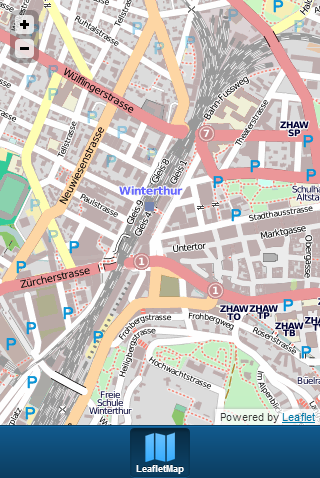
\includegraphics[scale=0.5]{images/implementation/leafletmap-screenshot}
	\caption{Leaflet Map-Komponente in Sencha Touch}
	\label{image-leafletmap-screenshot}
\end{figure}

\subsection{Verfügbarkeit}
Unsere Sencha Touch Komponente war schlussendlich so ausgereift, dass wir uns entschieden diese für die Allgemeinheit zugänglich zu machen.
Wir veröffentlichten sie deshalb unter dem Namen \emph{Ext.ux.LeafletMap} im offiziellen Sencha Market\footnote{\url{http://market.sencha.com/}}.
Sie ist verfügbar unter:

\begin{table}[H]
\centering
\begin{tabular}{|p{0.2\twocelltabwidth}|p{0.8\twocelltabwidth}|}
\hline 
\textbf{Ort} & \textbf{URL} \\ 
\hline 
Sencha Market & \url{https://market.sencha.com/users/162/extensions/177} \\ 
\hline 
GitHub & \url{https://github.com/tschortsch/Ext.ux.LeafletMap} \\ 
\hline 
\end{tabular} 
\caption{Ext.ux.LeafletMap Verfügbarkeit}
\label{leafletmap-availiblity}
\end{table}

\begin{figure}[H]
	\centering
	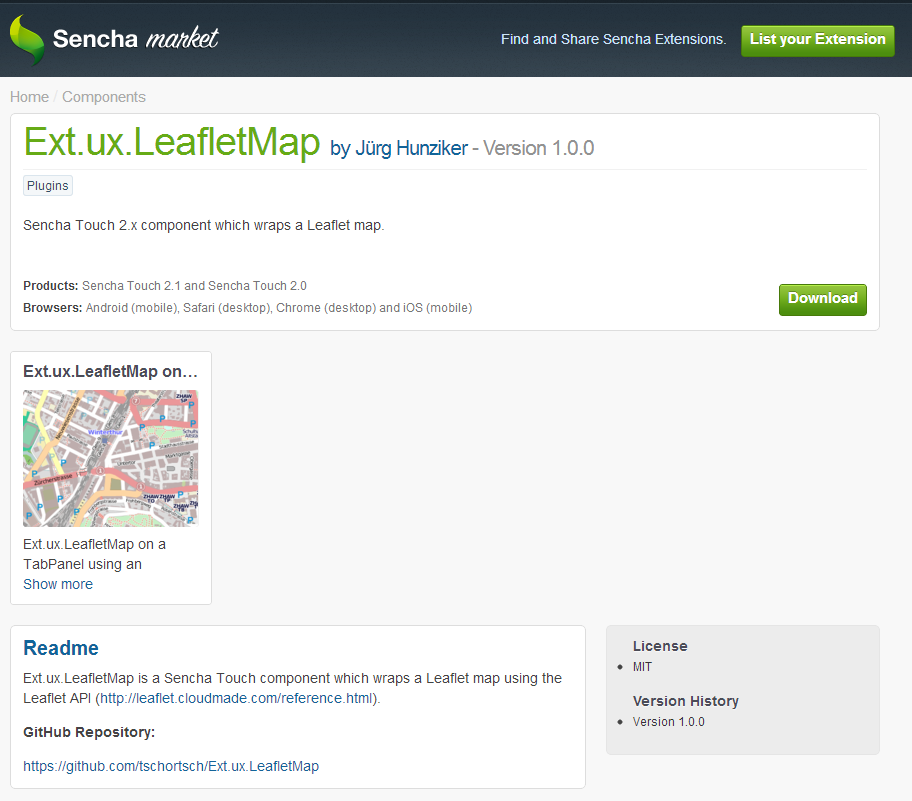
\includegraphics[scale=0.6]{images/implementation/leafletmap-sencha-market}
	\caption{Leaflet Map-Komponente im Sencha Market}
	\label{image-leafletmap-sencha-market}
\end{figure}

\subsection{Dokumentation}
Die Komponente ist durchgängig mit der Sencha-eigenen JavaScript-Dokumentationsprache \emph{JSDuck}\footnote{\url{https://github.com/senchalabs/jsduck}} dokumentiert. Die Dokumentation findet sich unter: \url{http://kort.herokuapp.com/docs/Ext.ux.LeafletMap}